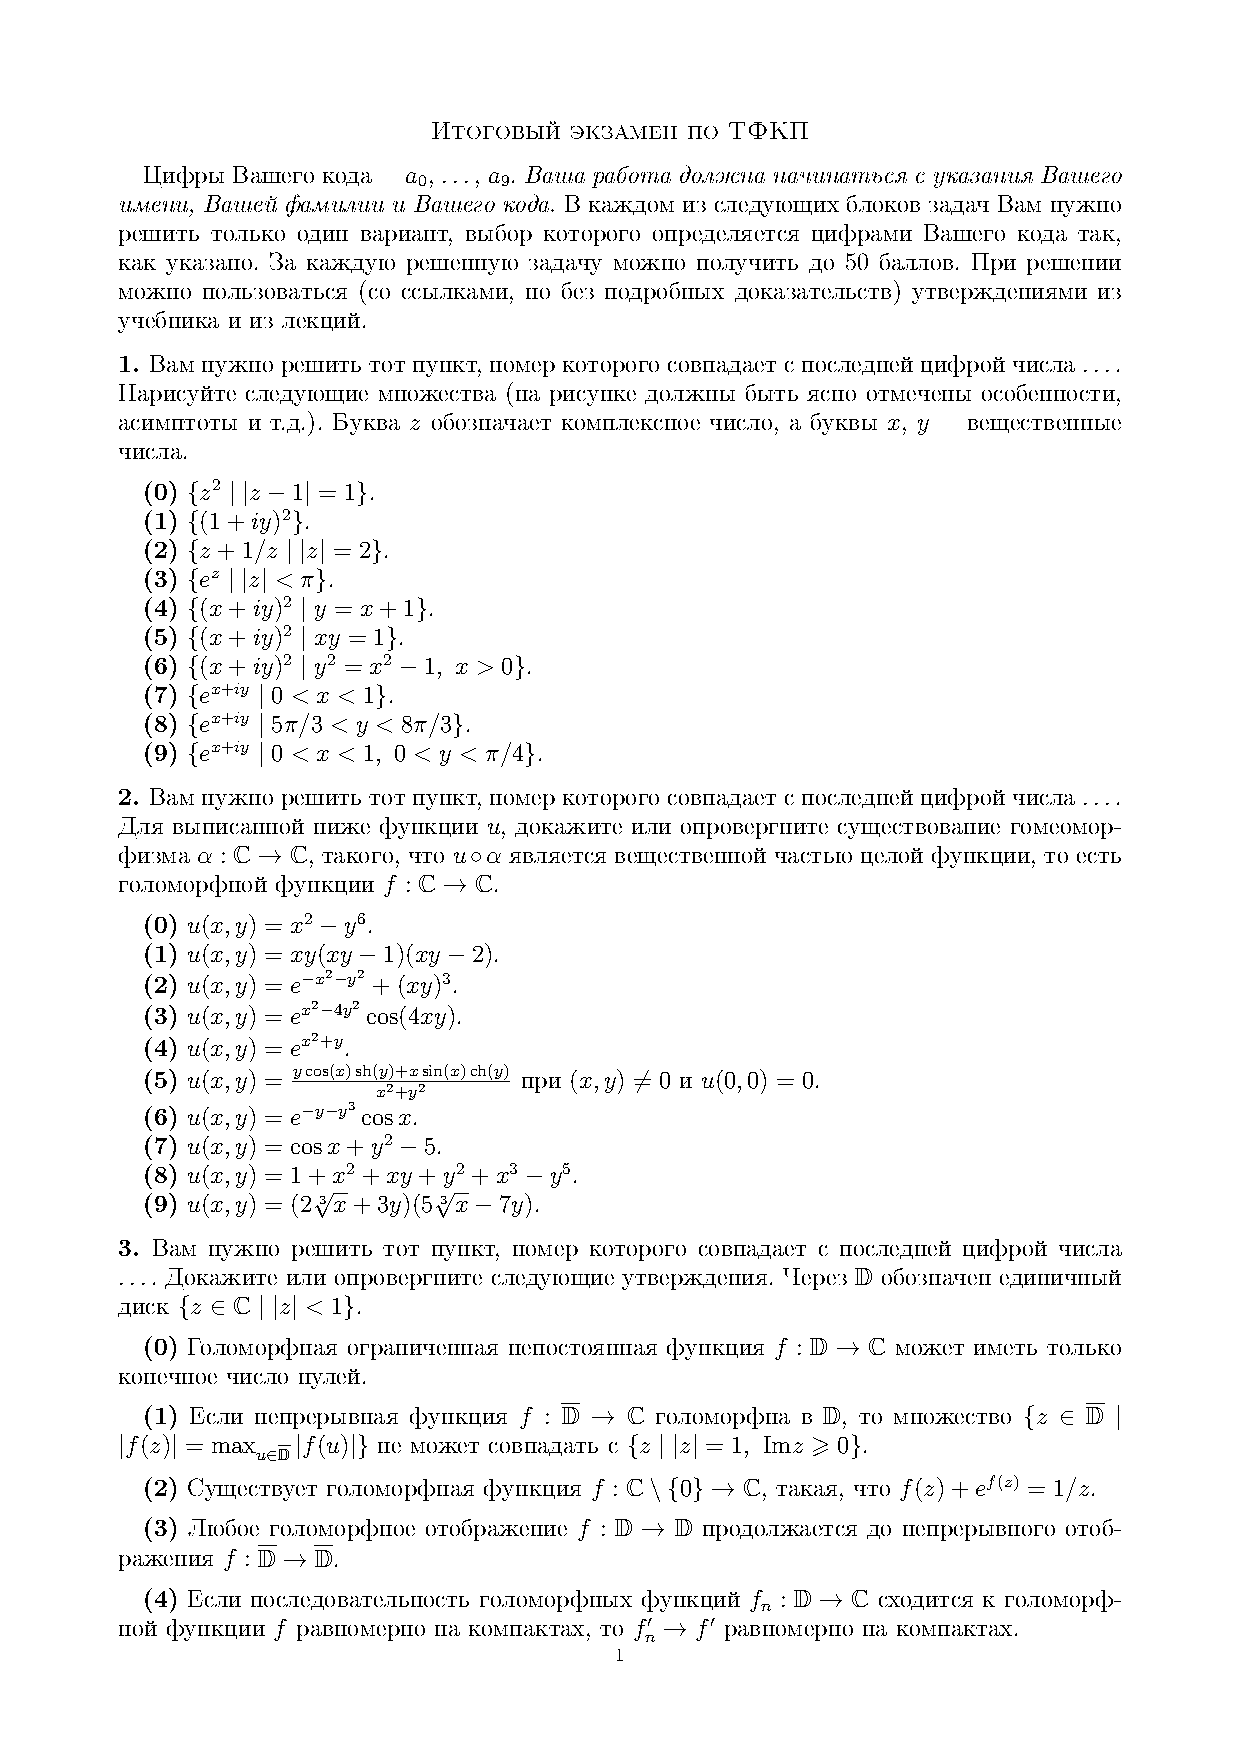
\includepdf[scale=1,pages=1-3]{Tasks/exam}
\newpage
\section*{Решения}
\subsection*{Задача 1}
	\begin{figure}[!h]
		\begin{minipage}[h]{0.49\linewidth}
			\center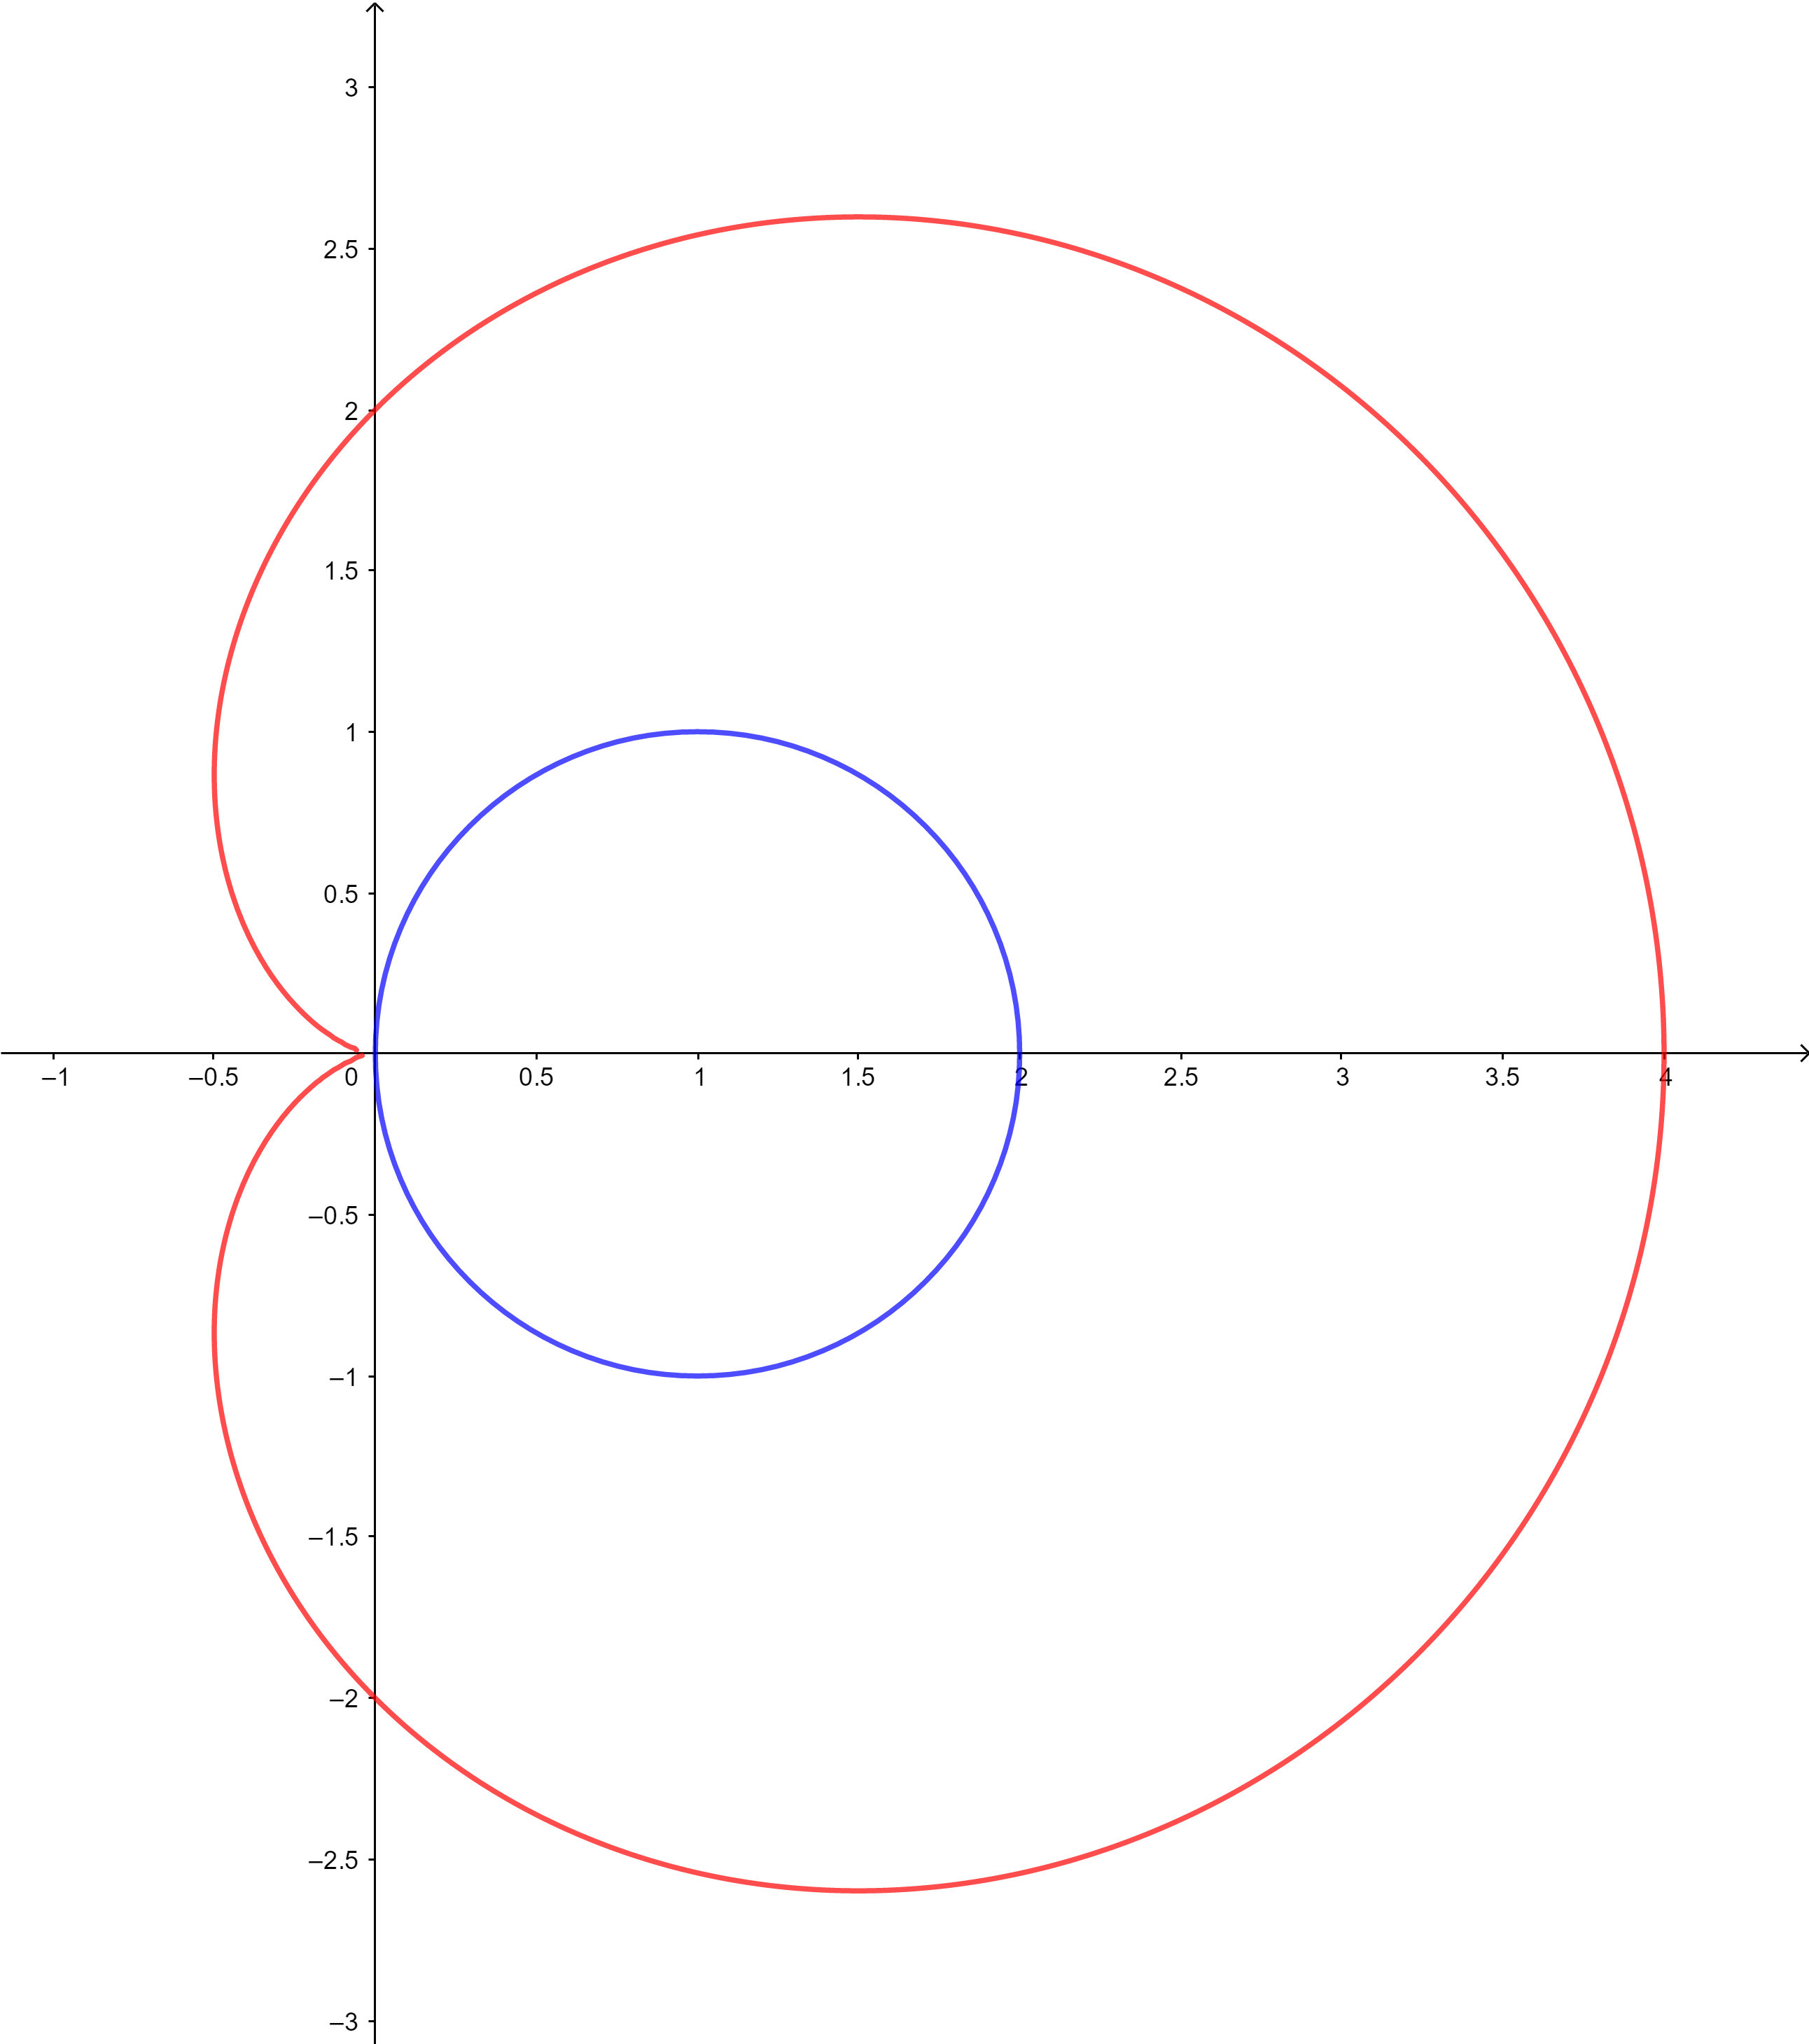
\includegraphics[width=0.9\linewidth]{10}
			\caption{$\{z^2|\ |z-1| = 1\}$}
		\end{minipage}
		\begin{minipage}[h]{0.49\linewidth}
			\center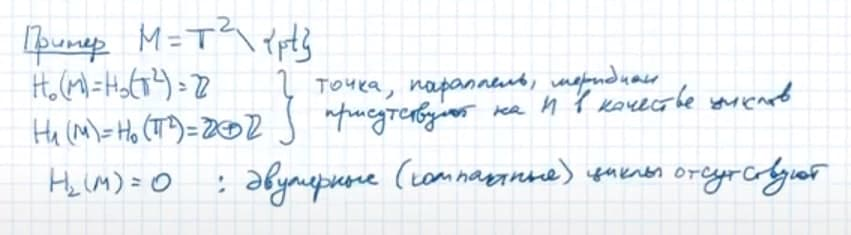
\includegraphics[width=0.9\linewidth]{11}
			\caption{$\{(1+iy)^2)\}$}
		\end{minipage}
	\end{figure}

	\begin{figure}[!h]
		\begin{minipage}[h]{0.49\linewidth}
			\center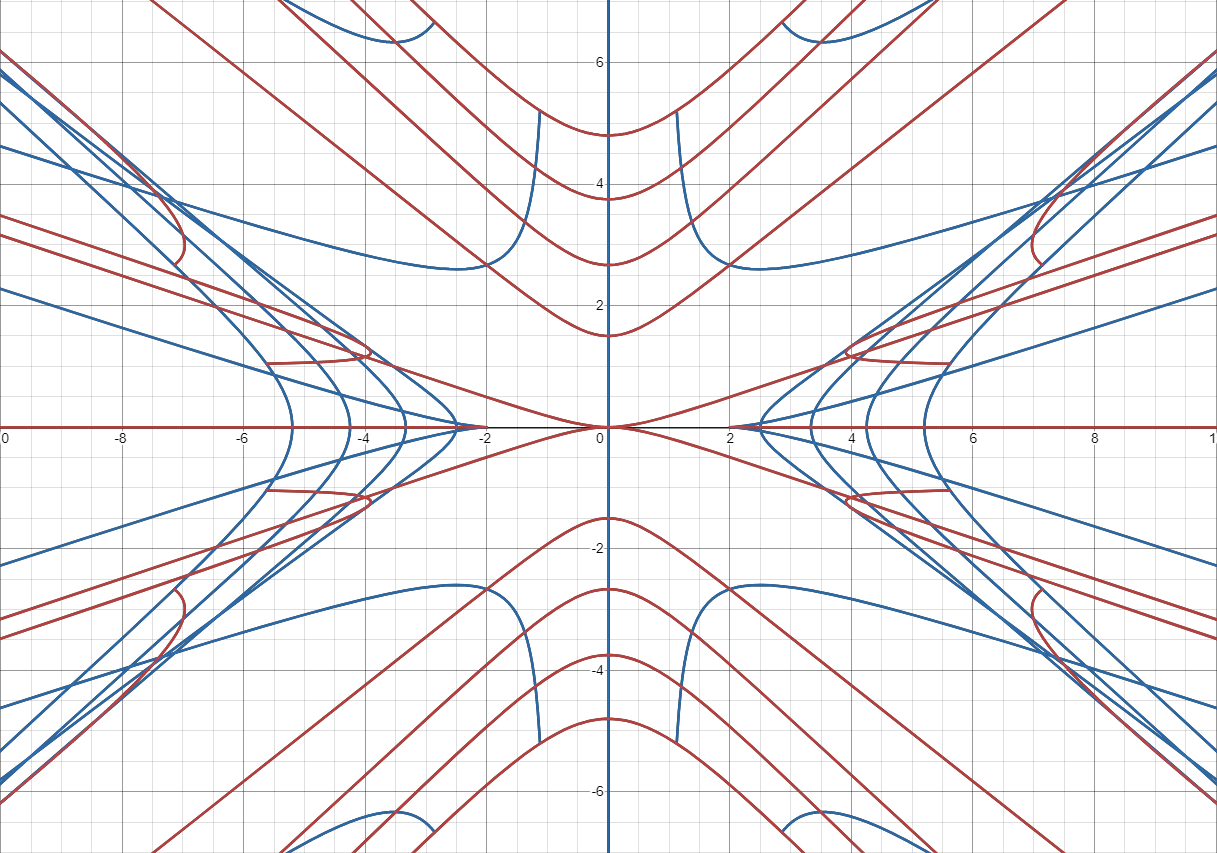
\includegraphics[width=0.9\linewidth]{12}
			\caption{$\{z+1/z|\ |z| = 2\}$}
		\end{minipage}
		\begin{minipage}[h]{0.49\linewidth}
			\center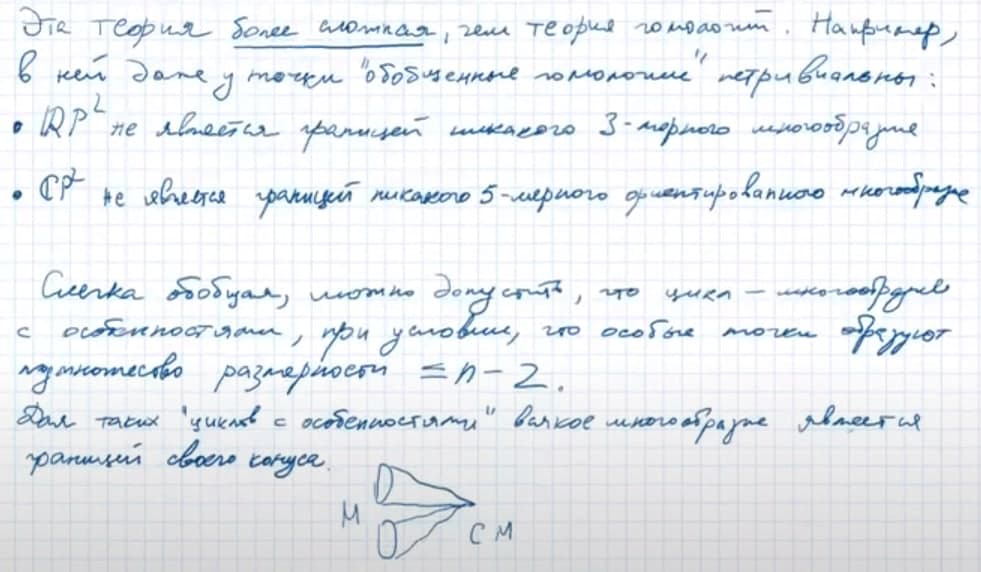
\includegraphics[width=0.9\linewidth]{13}
			\caption{$\{e^z|\ |z| < \pi\}$}
		\end{minipage}
	\end{figure}

	\begin{figure}[!h]
		\begin{minipage}[h]{0.49\linewidth}
			\center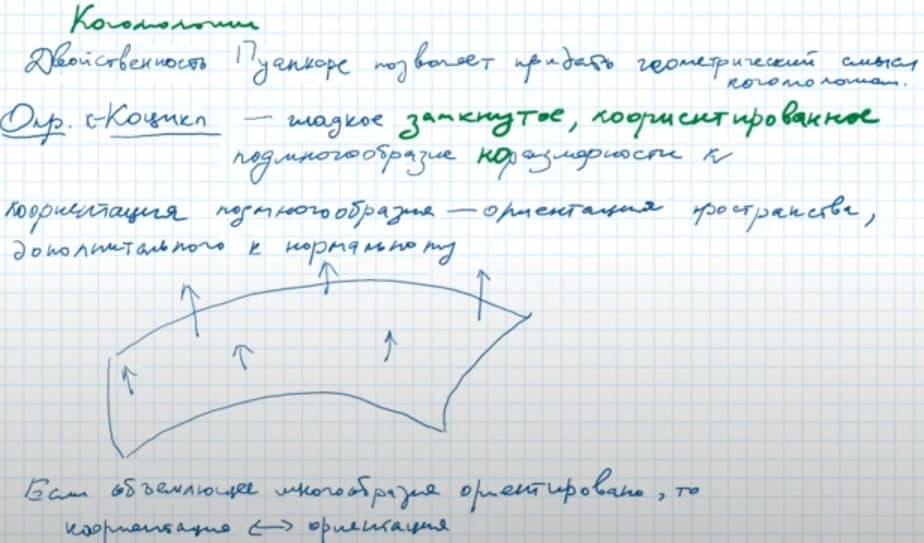
\includegraphics[width=0.75\linewidth]{14}
			\caption{$\{(x+iy)^2|\ y = x+1\}$}
		\end{minipage}
		\begin{minipage}[h]{0.49\linewidth}
			\center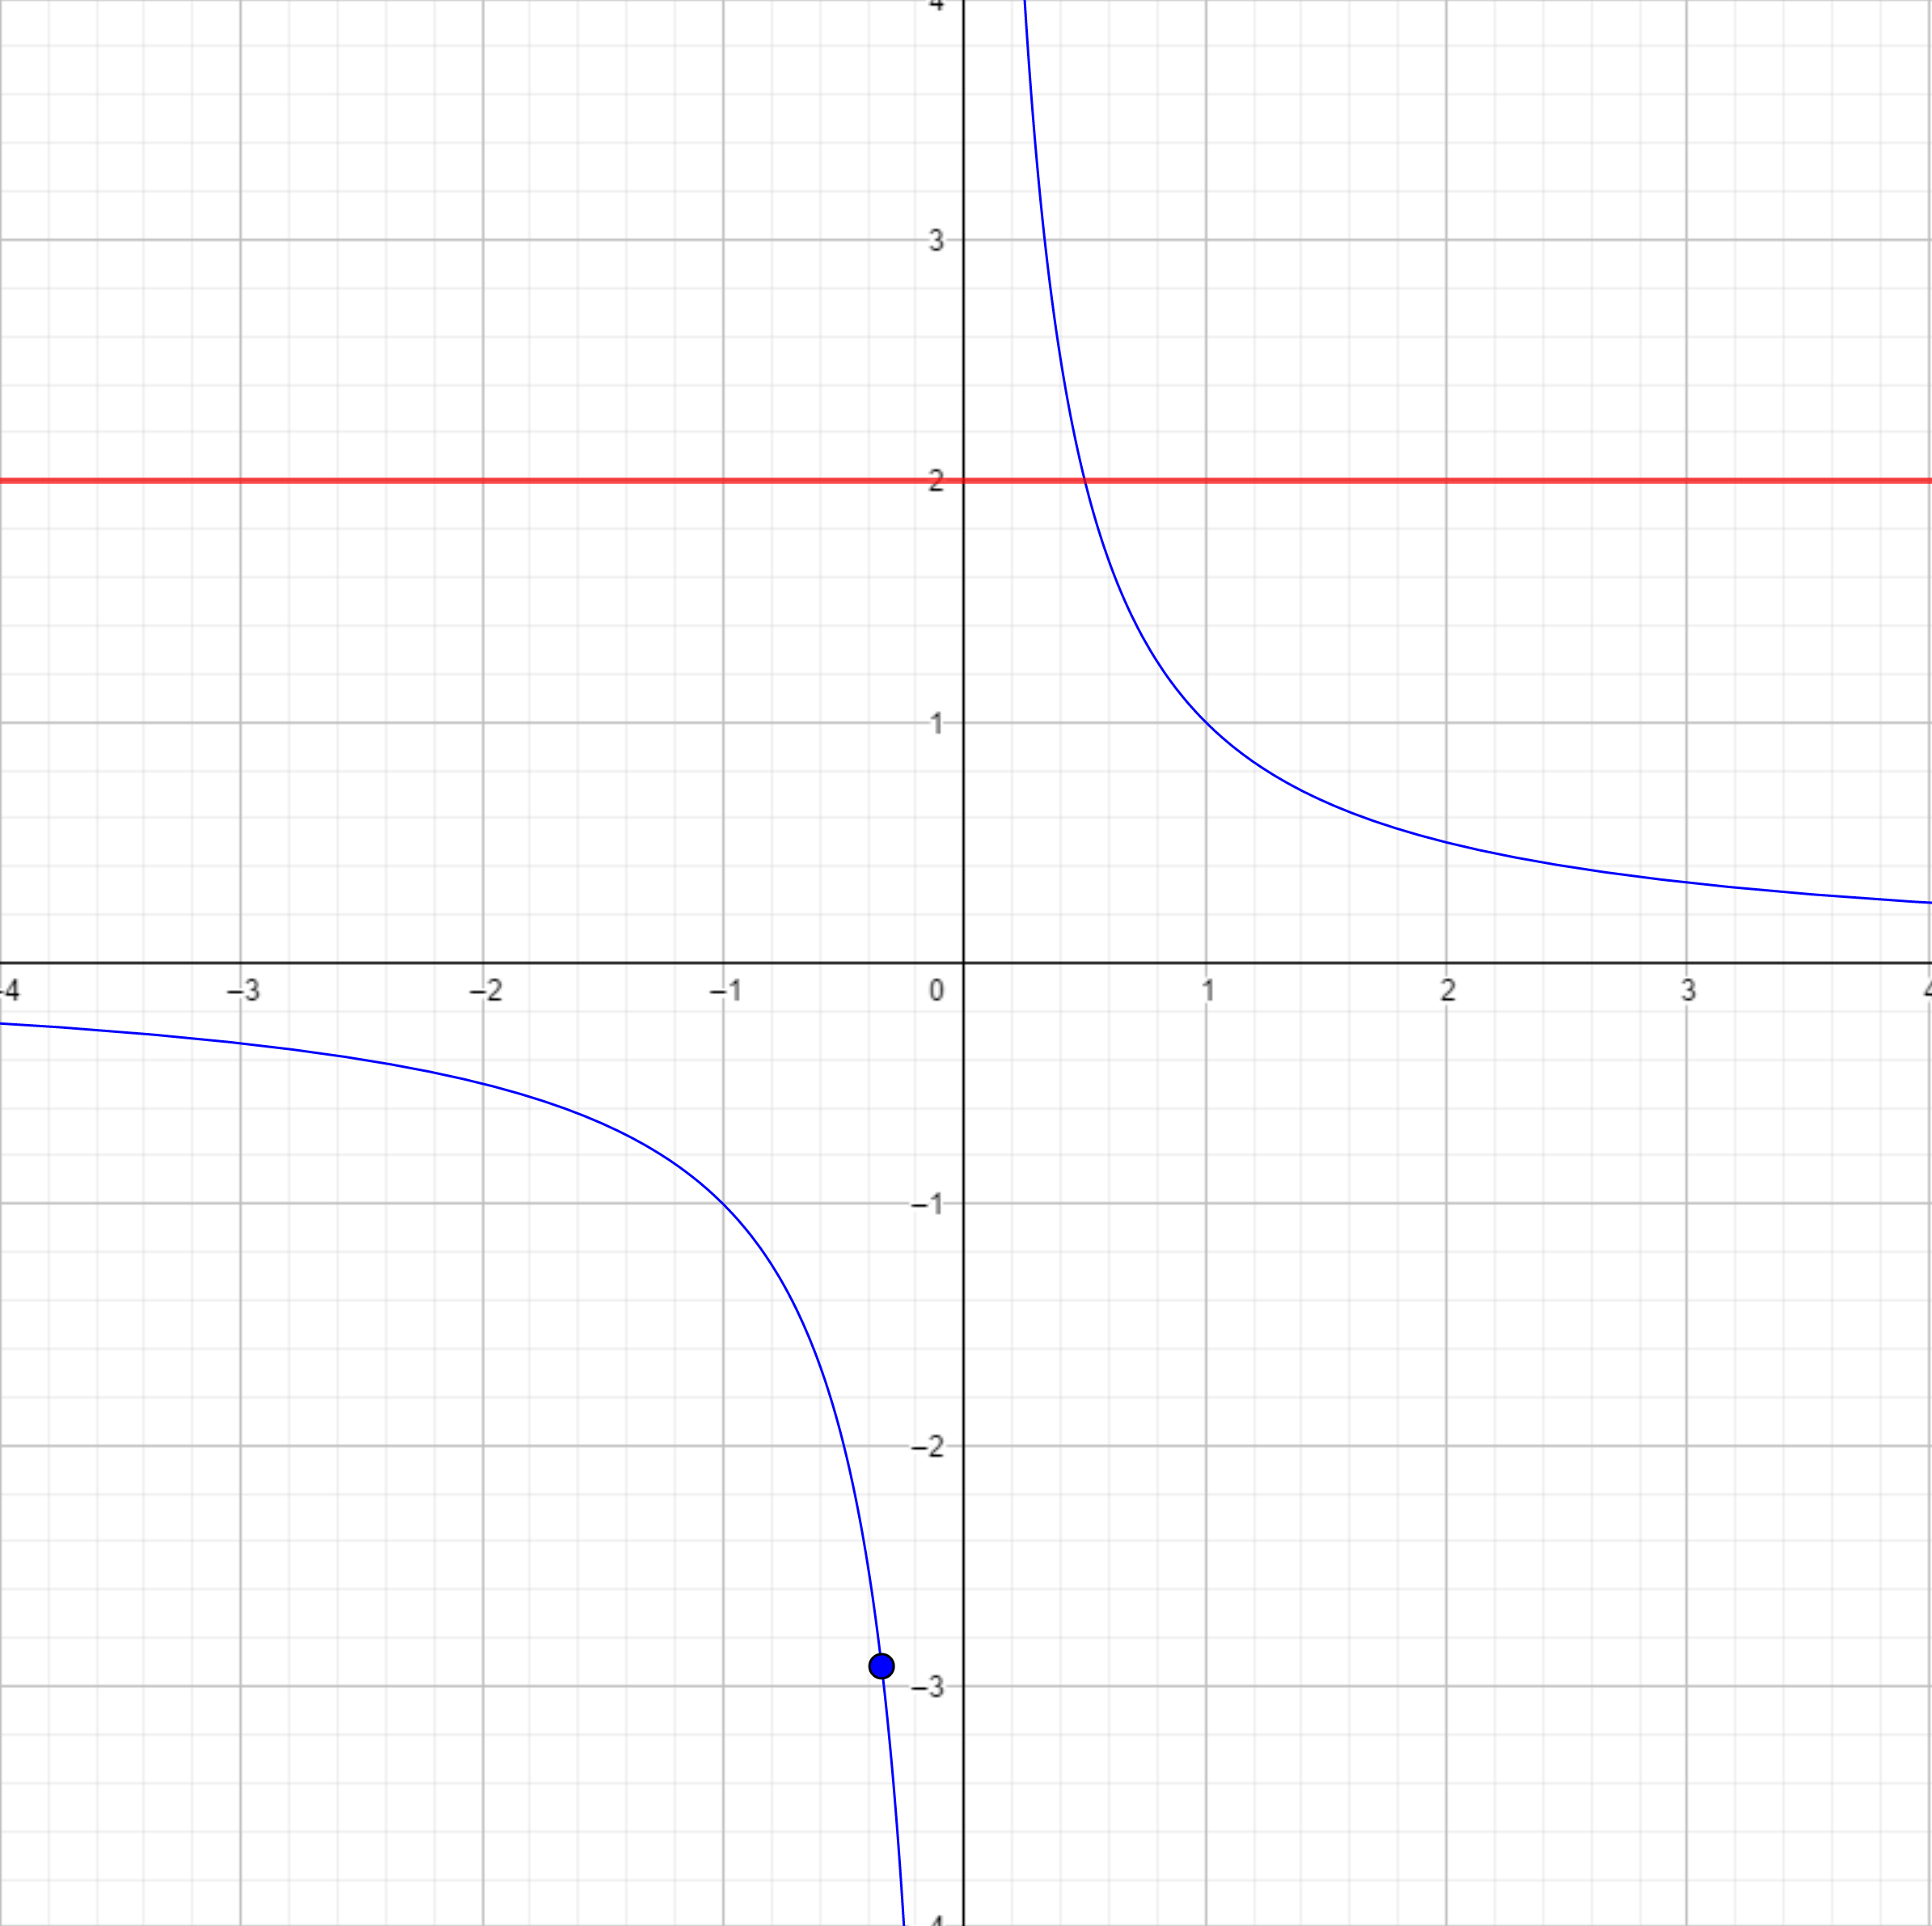
\includegraphics[width=0.75\linewidth]{15}
			\caption{$\{(x+iy)^2|\ xy=1\}$}
		\end{minipage}
	\end{figure}

	\begin{figure}[!h]
		\begin{minipage}[h]{0.49\linewidth}
			\center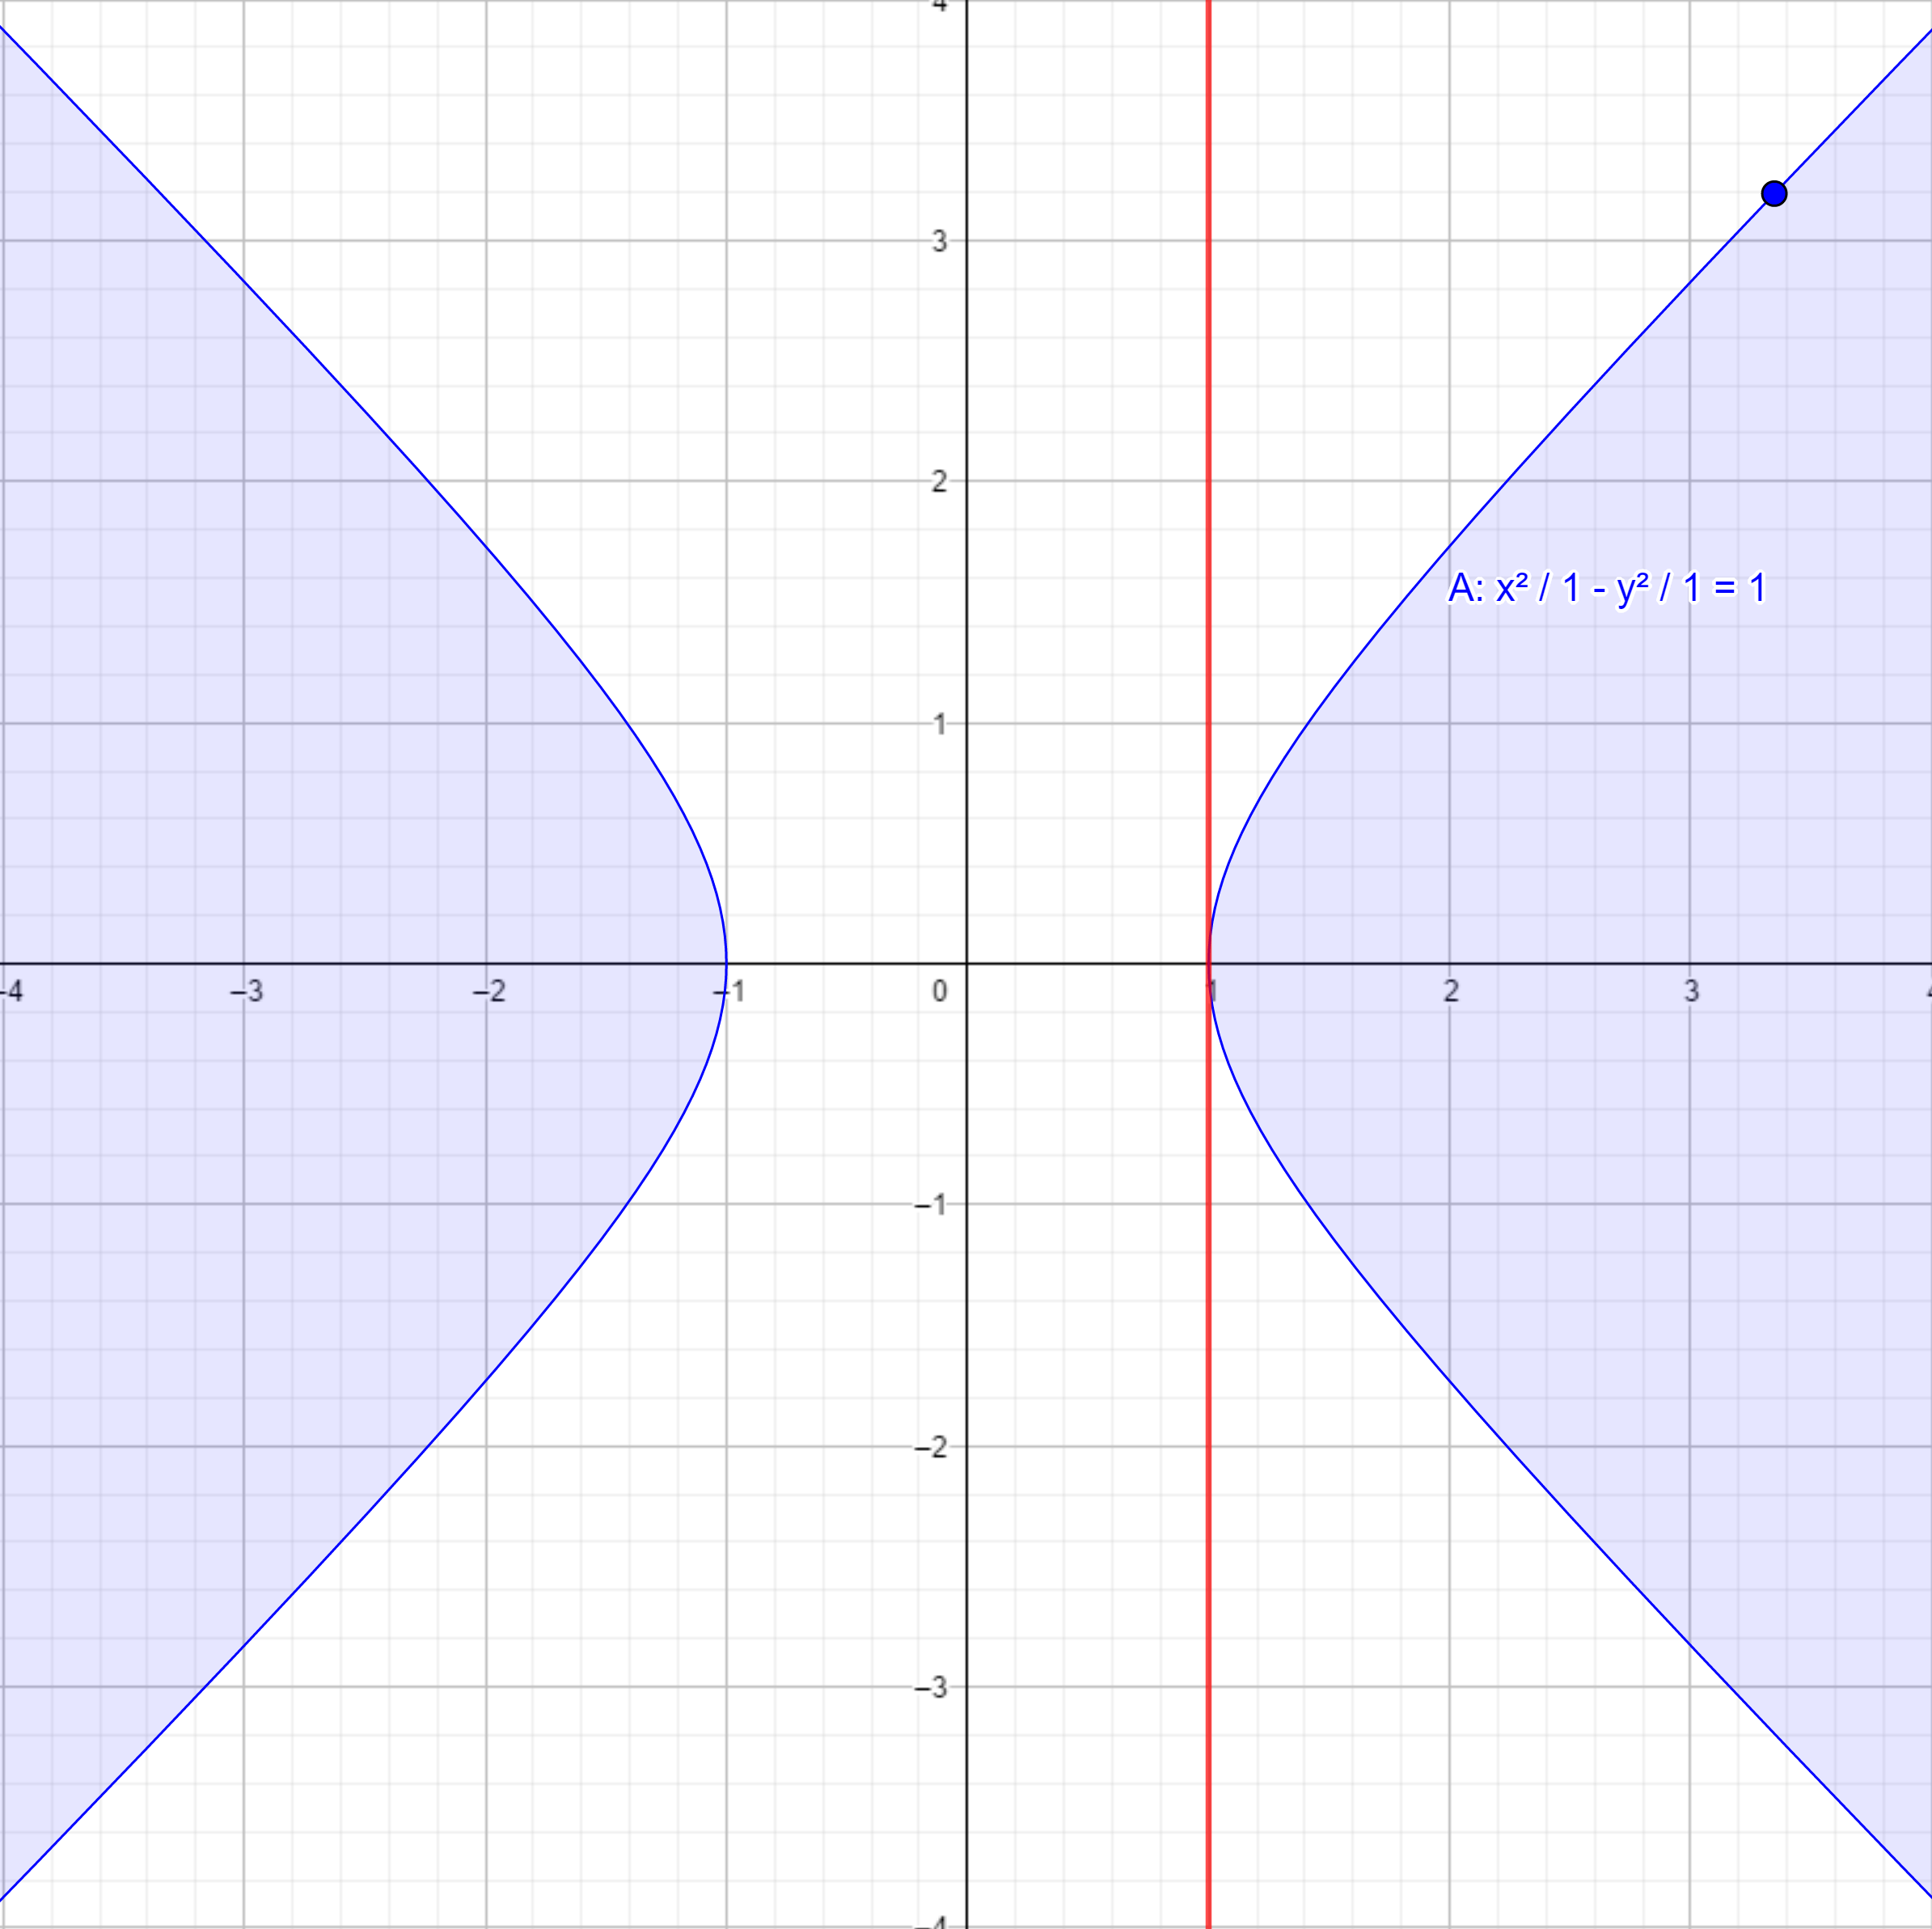
\includegraphics[width=0.75\linewidth]{16}
			\caption{$\{(x+iy)^2|\ y^2 = x^2 - 1, x>0\}$}
		\end{minipage}
		\begin{minipage}[h]{0.49\linewidth}
			\center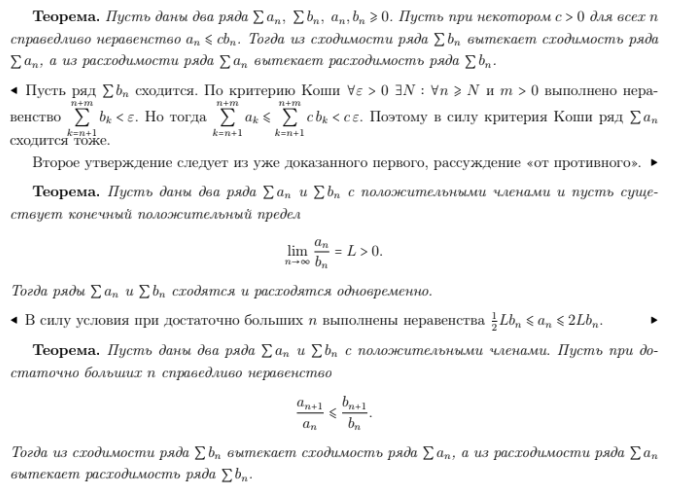
\includegraphics[width=0.75\linewidth]{17}
			\caption{$\{e^{x+iy}|\ 0<x<1\}$}
		\end{minipage}
	\end{figure}

	\begin{figure}[!h]
		\begin{minipage}[h]{0.49\linewidth}
			\center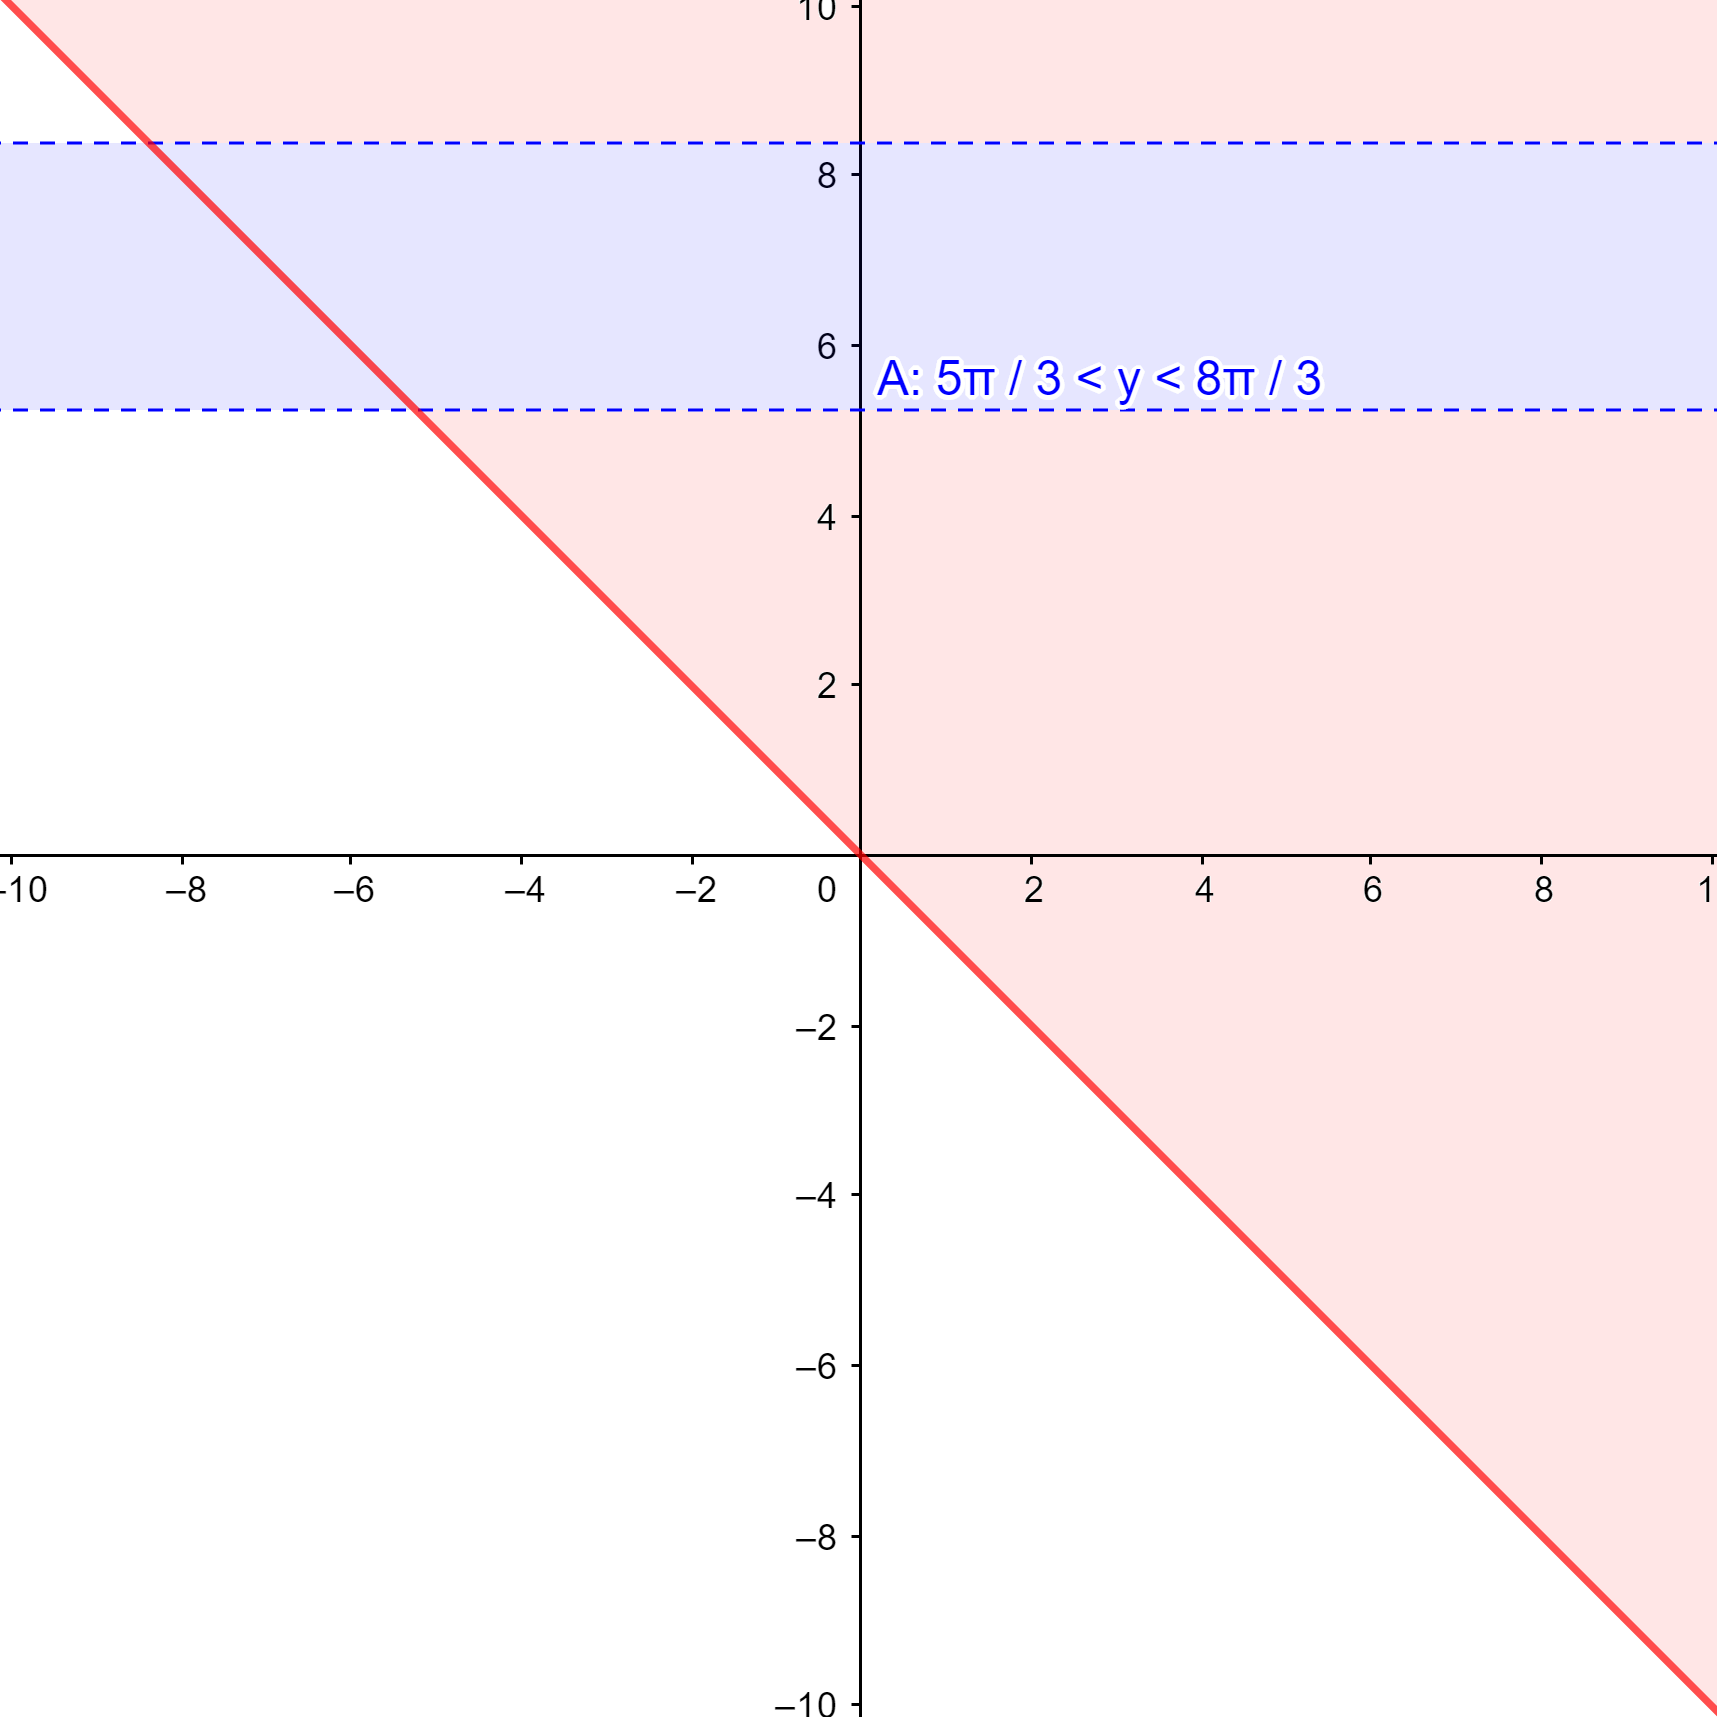
\includegraphics[width=0.75\linewidth]{18}
			\caption{$\{e^{x+iy}|\ 5\pi/3 < y < 8\pi/3\}$}
		\end{minipage}
		\begin{minipage}[h]{0.49\linewidth}
			\center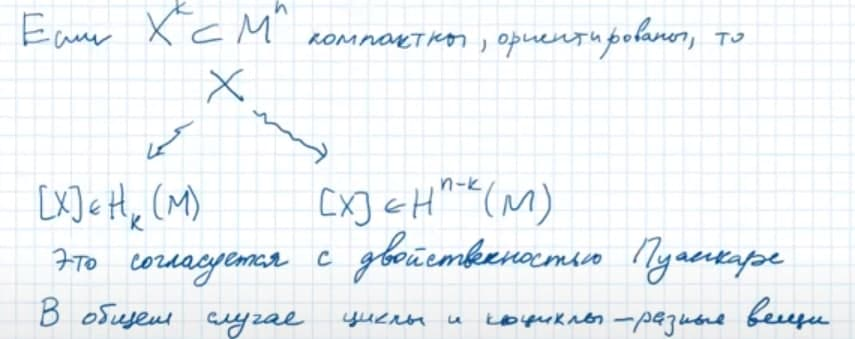
\includegraphics[width=0.75\linewidth]{19}
			\caption{$\{e^{x+iy}|\ 0<x<1, 0<y<\pi/4\}$}
		\end{minipage}
	\end{figure}
\newpage


\subsection*{Задача 2}
\subsubsection*{пункт 0}
	\begin{gather*}
		\alpha: (x,y) \mapsto (x, \sqrt[3]{y})\\
		u \circ \alpha (x,y) = x^2 - y^2 = \Re((x+iy)^2)
	\end{gather*}
\subsubsection*{пункт 3}
	\begin{gather*}
		\Re(e^{(x+iy)^2}) = \Re(e^{x^2 - y^2}(\cos(2xy) + i \sin(2xy))) = e^{x^2 - y^2} \cos(2xy)\\
		\alpha: (x,y) \mapsto (x, \frac{y}{2})\\
		u \circ \alpha = e^{x^2 - y^2} \cos(2xy) = \Re(e^{(x+iy)^2})
	\end{gather*}
\subsubsection*{пункт 4}
	По малой теореме Пикара область значений вещественной части целой функции - вся вещественная прямая. Но для любого гомеоморфизма $\alpha$ область значений $u \circ \alpha$ вложена в $\mathbb{R}^{+}$, следовательно подходящего $\alpha$ не существует
\subsubsection*{пункт 6}
	\begin{gather*}
		g^{-1}(y): y \mapsto y^3 + y\\
		\alpha: (x,y) \mapsto (x, g(y))\\
		u \circ \alpha = e^{-y} \cos(x) = \Re(e^{ix - y}) = \Re(e^{i(x+iy)})
	\end{gather*}
\subsubsection*{пункт 9}
	\begin{gather*}
		\alpha: (x,y) \mapsto (x^3 2.1^{\frac{3}{2}}, y)\\
		u \circ \alpha = (2x \cdot \sqrt{2.1} + 3y)(5x \sqrt{2.1} - 7y)
		= 21x^2 - 21y^2 + \sqrt{2.1}xy\\
		= \Re(21(x+iy)^2 - i \frac{\sqrt{2.1}}{2}(x+iy)^2)
		= \Re((x+iy)^2(21 - i \frac{\sqrt{2.1}}{2}))
	\end{gather*}
\vskip 0.4in

\subsection*{Задача 5}
\subsubsection*{пункт 0}
	\begin{gather*}
		f: z^5\quad g: 5z^2 + 2z + 1\\
		|z|=2:\ g \leqslant 5 \cdot 2^2 + 2 \cdot 2 + 1 = 25\quad f = 2^5 = 32,\ 25 < 32\\
		g: z^5\quad f: 5z^2 + 2z + 1\\
		|z|=1:\ g = 1\quad f \leqslant 5 + 2 + 1 = 8,\ 1 < 8\\
		5 - 1 = 4
	\end{gather*}
\subsubsection*{пункт 1}
	\begin{gather*}
		\left|\frac{e^z}{z}\right| \leqslant e < 3 \leqslant |3z^9|\\
		g(z) = 3z^9,\quad \text{то есть корней } 9
	\end{gather*}
\subsubsection*{пункт 3}
	Заметим что $f(-5) < 0, f(-4) > 0, f(0) < 0, f(1) > 0$, следовательно есть 3 вещественных корня, остальные корни имеют вид $\alpha \pm \beta i$, а так как сумма вещественных корней отрицательна и перед $z^4$ стоит 0, то сумма всех корней ноль, а следовательно оставшиеся 2 комплексных корня имеют положительную вещественную часть.
\subsubsection*{пункт 5}
	\begin{gather*}
		f: z^7 + z^3 + 1\quad g: z^4 + z^3\\
		|z| = 2:\ |g(z)| = 2^4 + 2^3 < 2^7 - 2^3 - 1 \leqslant |f(z)|\\
		\gamma_1 = \{z = x+iy: 0 \leqslant x \leqslant 2, y = 0\}\quad \min(f(x) - g(x)) > 0\\
		\gamma_2 = \{z: |z| = 2, 0 \leqslant \arg z \leqslant \frac{\pi}{2}\}\\
		\gamma_3 = \{z = x + iy: x = 0, 0 \leqslant y \leqslant 2\} 
	\end{gather*}
\subsubsection*{пункт 6}
	\begin{gather*}
		g: z^3\quad f: z + 1\\
		|z|= \frac{1}{2}:\ f \leqslant \frac{1}{2} + 1 = \frac{3}{2}\quad g = \frac{1}{2}^{3} = \frac{1}{8},\ \frac{1}{8} < \frac{3}{2}
	\end{gather*}
\subsubsection*{пункт 7}
	\begin{gather*}
		f: z^6\quad g: -8z + 10\\
		|z|=3:\ g \leqslant -8 \cdot 3 + 10 = -14 \quad f = 3^6 = 729,\ -14 < 729\\
		g: z^6\quad f: -8z + 10\\
		|z|=1:\ g = 1\quad f \leqslant -8 + 10 = 2,\ 1 < 2\\
		6 - 1 = 5
	\end{gather*}
\subsubsection*{пункт 8}
	\begin{gather*}
		f: z^4\quad g: -5z + 1\\
		|z|=2:\ g \leqslant -5 \cdot 2 + 1 = -9 \quad f = 2^4 = 16,\ -9 < 16\\
		|z|=1:\ g \leqslant -5 + 1 = -4 \quad f = 1,\ -4 < 1\\
		4 - 1 = 3
	\end{gather*}
\subsubsection*{пункт 9}
	\begin{gather*}
		z^6 - z^5 + z^3 - z + 1 = (z^2 - z + 1)(z^4 - z^2 + 1)\\
		z^2 - z + 1 = 0: (-1)^{1/3}, -(-1)^{2/3}
	\end{gather*}